\chapter{\basisDimTitle}\label{basisdimension}

\label{sec:dimension}
\label{dimension}
In chapter~\ref{linearind}, the notions of   a linearly independent set of vectors in a vector space $V$, and of a set of vectors that span $V$ were established; any set of vectors that span $V$ can be reduced to some minimal collection of linearly independent vectors; such a minimal set is called a \emph{basis} of the subspace $V$.  

\begin{definition}
Let $V$ be a vector space.  Then a set $S$ is a {\bf basis}\index{Basis} for $V$ if $S$ is linearly independent and $V=\spa S$.


If $S$ is a basis of $V$ and $S$ has only finitely many elements, then we say that $V$ is {\bf finite-dimensional}.  The number of vectors in $S$ is the {\bf dimension}\index{Dimension} of~$V$.
\end{definition}

Suppose $V$ is a \emph{finite-dimensional}\index{Vector space!finite dimensional} vector space, and $S$ and $T$ are two different bases for $V$.  One might worry that $S$ and $T$ have a different number of vectors; then we would have to talk about the dimension of $V$ in terms of the basis $S$ or in terms of the basis $T$.  Luckily this isn't what happens.
Later in this chapter, we will show that $S$ and $T$ must have the same number of vectors.  This means that the dimension of a vector space is basis-independent.  In fact, dimension is a very important  characteristic of a vector space.% $V$.

\begin{example}
$P_n(t)$ (polynomials in $t$ of degree $n$ or less) has a basis $\{1,t,\ldots , t^n \}$, since every vector in this space is a sum
\[
a^0\,1+a^1\,t+\cdots +a^n\,t^n, \qquad a^i\in \Re\, ,
\]
so $P_n(t)=\spa \{1,t,\ldots , t^n \}$.  This set of vectors is linearly independent;  If the polynomial $p(t)=c^01+c^1t+\cdots +c^nt^n=0$, then $c^0=c^1=\cdots =c^n=0$, so $p(t)$ is the zero polynomial.  
Thus $P_n(t)$ is finite dimensional, and $\dim P_n(t)=n+1$.
\end{example}



\begin{theorem}\label{uniqvec}
Let $S=\{v_1, \ldots, v_n \}$  be a basis for a vector space $V$.  Then every vector $w \in V$ can be written \emph{uniquely} as a linear combination of vectors in the basis $S$:
\[
w=c^1v_1+\cdots + c^nv_n.
\]
\end{theorem}

\begin{proof}
Since $S$ is a basis for $V$, then $\spa S=V$, and so there exist constants~$c^i$ such that $w=c^1v_1+\cdots + c^nv_n$.

Suppose there exists a second set of constants $d^i$ such that 
$$w=d^1v_1+\cdots + d^nv_n\, .$$  Then
\begin{eqnarray*}
0_V&=&w-w\\
&=&c^1v_1+\cdots + c^nv_n-d^1v_1-\cdots - d^nv_n \\[1mm]
&=&(c^1-d^1)v_1+\cdots + (c^n-d^n)v_n. \\
\end{eqnarray*}
If it occurs exactly once that $c^i\neq d^i$, then the equation reduces to $0=(c^i-d^i)v_i$, which is a contradiction since the vectors $v_i$ are assumed to be non-zero.

If we have more than one $i$ for which $c^i\neq d^i$, we can use this last equation to write one of the vectors in $S$ as a linear combination of other vectors in $S$, which contradicts the assumption that $S$ is linearly independent.  Then for every $i$, $c^i=d^i$.
\end{proof}

\Videoscriptlink{basis_and_dimension_thm.mp4}{Proof Explanation}{basis_and_dimension_thm}

\begin{remark}
This theorem is the one that makes bases so useful--they allow us to convert abstract vectors into column vectors.
By ordering the set $S$ we obtain $B=(v_1,\ldots,v_n)$ and can write
$$
w=(v_1,\ldots,v_n) \ccolvec{c^1\\ \vdots\\ c^n }=\ccolvec{c^1\\ \vdots\\ c^n }_B\, .
$$
Remember that in general it makes no sense to drop the subscript $B$ on the column vector on the right--most vector spaces  are not made from  columns of numbers!
\end{remark}

\Videoscriptlink{eigenvectors_and_eigenvalues_matrix.mp4}{Worked Example}{scripts_eigenvalseigenvects_matrix}

Next, we would like to establish a method for determining whether a collection of vectors forms a basis for $\Re^n$.  But first, we need to show that any two bases for a finite-dimensional vector space has the same number of vectors.

\begin{lemma}\label{mlessn}
If $S=\{v_1, \ldots, v_n \}$ is a basis for a vector space $V$ and $T=\{w_1, \ldots, w_m \}$ is a linearly independent set of vectors in $V$, then $m\leq n$.
\end{lemma}

%\begin{figure}
%\begin{center}
%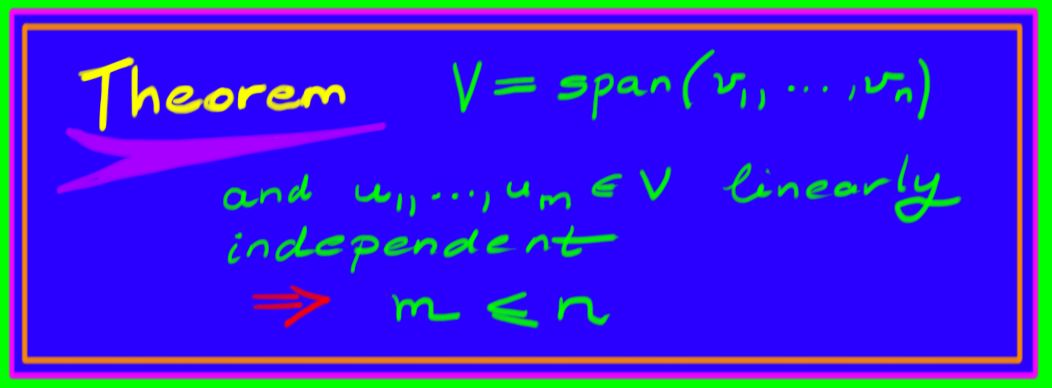
\includegraphics[scale=.28]{\basisDimPath/indep_span.jpg}
%\end{center}
%\end{figure}

The idea of the proof is to start with the set $S$ and replace vectors in $S$ one at a time with vectors from $T$, such that after each replacement we still have a basis for $V$.

%\begin{center}\href{\webworkurl ReadingHomework17/1/}{Reading homework: problem \ref{basisdimension}.1}\end{center}
\Reading{BasisAndDimension}{1}

\begin{proof}
Since $S$ spans $V$, then the set $\{w_1, v_1, \ldots, v_n \}$ is linearly dependent.  Then we can write $w_1$ as a linear combination of the $v_i$; using that equation, we can express one of the $v_i$ in terms of $w_1$ and the remaining $v_j$ with~$j\neq i$.  Then we can discard one of the $v_i$ from this set to obtain a linearly independent set that still spans $V$.  Now we need to prove that $S_1$ is a basis; we must show that $S_1$ is linearly independent and that $S_1$ spans $V$.

The set $S_1=\{w_1, v_1, \ldots, v_{i-1}, v_{i+1},\ldots, v_n \}$ is linearly independent:  By the previous theorem, there was a unique way to express $w_1$ in terms of the set~$S$.  Now, to obtain a contradiction, suppose there is some $k$ and constants~$c^i$ such that
\[
v_k = c^0w_1+c^1v_1+\cdots + c^{i-1}v_{i-1} + c^{i+1}v_{i+1} + \cdots + c^nv_n.
\]
Then replacing $w_1$ with its expression in terms of the collection $S$ gives a way to express the vector $v_k$ as a linear combination of the vectors in $S$, which contradicts the linear independence of $S$.  On the other hand, we cannot express $w_1$ as a linear combination of the vectors in $\{v_j | j\neq i\}$, since the expression of $w_1$ in terms of $S$ was unique, and had a non-zero coefficient for the vector $v_i$.  Then no vector in $S_1$ can be expressed as a combination of other vectors in $S_1$, which demonstrates that $S_1$ is linearly independent.

The set $S_1$ spans $V$:  For any $u\in V$, we can express $u$ as a linear combination of vectors in $S$.  But we can express $v_i$ as a linear combination of vectors in the collection $S_1$; rewriting $v_i$ as such allows us to express $u$ as a linear combination of the vectors in $S_1$. Thus $S_1$ is a basis of $V$ with $n$ vectors.

We can now iterate this process, replacing one of the $v_i$ in $S_1$ with $w_2$, and so on.  If $m\leq n$, this process ends with the set $S_m=\{w_1,\ldots, w_m$, $v_{i_1},\ldots,v_{i_{n-m}}  \}$, which is fine.

Otherwise, we have $m>n$, and the set $S_n=\{w_1,\ldots, w_n \}$ is a basis for~$V$.  But we still have some vector 
$w_{n+1}$  in $T$ that is not in $S_n$.  Since $S_n$ is a basis, we can write $w_{n+1}$ as a combination of the vectors in $S_n$, which contradicts the linear independence of the set $T$.  Then it must be the case that $m\leq n$, as desired.
\end{proof}

\Videoscriptlink{basis_and_dimension_example.mp4}{Worked Example}{basis_and_dimension_example}

\begin{corollary}\label{corsame}
For a finite-dimensional vector space $V$, any two bases for~$V$ have the same number of vectors.
\end{corollary}

\begin{proof}
Let $S$ and $T$ be two bases for $V$.  Then both are linearly independent sets that span $V$.  Suppose $S$ has $n$ vectors and $T$ has $m$ vectors.  Then by the previous lemma, we have that $m\leq n$.  But (exchanging the roles of $S$ and $T$ in application of the lemma) we also see that $n\leq m$.  Then $m=n$, as desired.
\end{proof}

%\begin{center}\href{\webworkurl ReadingHomework17/2/}{Reading homework: problem \ref{basisdimension}.2}\end{center}
\Reading{BasisAndDimension}{2}

\section{Bases in $\Re^n$.}

In review question~\ref{stdbasis}, chapter~\ref{linearind} you checked that
\[
\Re^n = \spa \left\{ \colvec{1\\0\\ \vdots \\ 0}, 
\colvec{0\\1\\ \vdots \\ 0}, \ldots, \colvec{0\\0\\ \vdots \\ 1}\right\},
\]
and that this set of vectors is linearly independent. (If you didn't do that problem, check this before reading any further!)  So this set of vectors is a basis for~$\Re^n$, and $\dim \Re^n=n$.  This basis is often called the \emph{standard} or \emph{canonical basis}\index{Standard basis}\index{Canonical basis|seealso{Standard basis}} for $\Re^n$.  The vector with a one in the $i$th position and zeros everywhere else is written 
$e_i$. (You could also view it as the function $\{1,2,\ldots,n\}\to {\mathbb R}$ where $e_i(j)=1$ if $i=j$ and $0$ if $i\neq j$.)  It points in the direction of the $i$th coordinate axis, and has unit length.  In multivariable calculus classes, this basis is often written $\{ \hat i,\hat j,\hat k \}$ for $\Re^3$. 

%\begin{figure}
%\begin{center}
%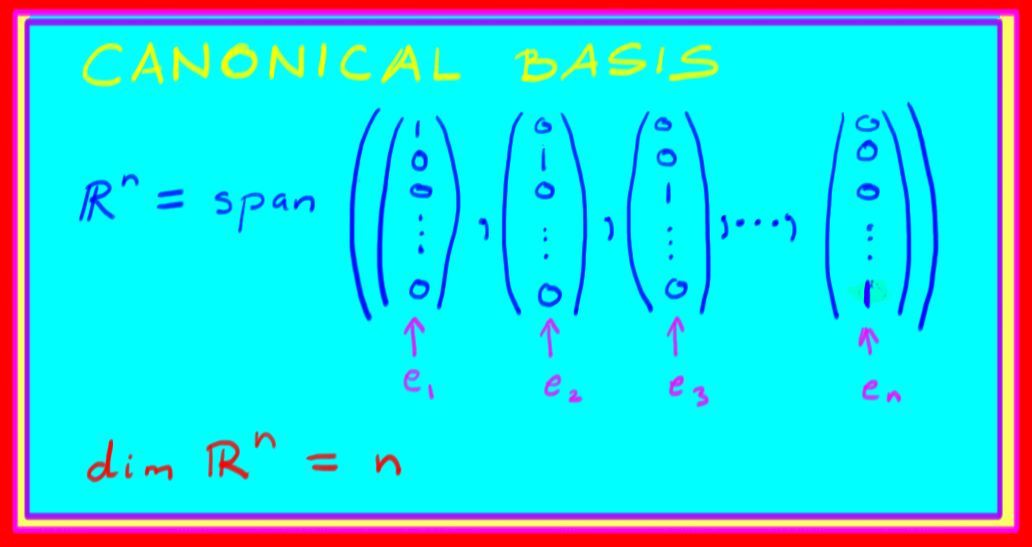
\includegraphics[scale=.32]{\basisDimPath/canonical.jpg}
%\end{center}
%\end{figure}

Note that it is often convenient to order  basis elements, so rather than writing a set
of vectors, we would write a list. This is called an ordered basis. For example, the canonical ordered basis for ${\mathbb R^n}$ is $(e_1,e_2,\ldots,e_n)$. The possibility to reorder basis vectors is not the only way in which bases are non-unique.

\begin{remark}[Bases are not unique.]
While there exists a unique way to express a vector in terms of any particular basis, bases themselves are far from unique.
For example, both of the sets 
\[
\left\{ \colvec{1\\0}, \colvec{0\\1} \right\} \text{ and }
\left\{ \colvec{1\\1}, \colvec{1\\-1} \right\}
\]
are bases for $\Re^2$.  Rescaling any vector in one of these sets is already enough to show that~$\Re^2$ has infinitely many bases.  But even if we require that all of the basis vectors have unit length, it turns out that there are still infinitely many bases for $\Re^2$ (see review question~\ref{lotsofbases}).
\end{remark}


To see whether a set of vectors $S=\{v_1, \ldots, v_m \}$ is a basis for~$\Re^n$, we have to check that the elements  are linearly independent and that they span~$\Re^n$.  From the previous discussion, we also know that $m$ must equal $n$, so lets assume~$S$ has $n$ vectors.
If $S$ is linearly independent, then there is no non-trivial solution of the equation
\[
0 = x^1v_1+\cdots + x^nv_n.
\]
Let $M$ be a matrix whose columns are the vectors $v_i$ and $X$ the column vector with entries $x^i$.  Then the above equation is equivalent to requiring that there is a unique solution to \[MX=0\, .\]

To see if $S$ spans $\Re^n$, we take an arbitrary vector $w$ and solve the linear system
\[
w=x^1v_1+\cdots + x^nv_n
\]
in the unknowns $x^i$.  For this, we need to find a unique solution for the linear system $MX=w$.  

Thus, we need to show that $M^{-1}$ exists, so that 
\[
X=M^{-1}w
\]
is the unique solution we desire.  Then we see that $S$ is a basis for $\mathbb{R}^n$ if and only if $\det M\neq 0$.




\begin{theorem}
Let $S=\{v_1, \ldots, v_m \}$ be a collection of vectors in $\Re^n$.  Let~$M$ be the matrix whose columns are the vectors in $S$.  Then $S$ is a basis for $V$ if and only if $m$ is the dimension of $V$ and 
\[
\det M \neq 0.
\]
\end{theorem}

\begin{remark}
Also observe that  $S$ is a basis if and only if ${\rm RREF}(M)=I$.
\end{remark}

\begin{example}
Let 
\[
S=\left\{ \colvec{1\\0}, \colvec{0\\1} \right\} \text{ and }
T=\left\{ \colvec{1\\1}, \colvec{1\\-1} \right\}.
\]
Then set $M_S=\begin{pmatrix}
1 & 0\\
0 & 1\\
\end{pmatrix}$.  Since $\det M_S=1\neq 0$, then $S$ is a basis for $\Re^2$.\\

\noindent
Likewise, set $M_T=\begin{pmatrix}
1 & 1\\
1 & -1\\
\end{pmatrix}$.  Since $\det M_T=-2\neq 0$, then $T$ is a basis for $\Re^2$.
\end{example}


\section{Matrix of a Linear Transformation (Redux)}\index{Matrix of a linear transformation}

Not only do bases allow us to describe arbitrary vectors as column vectors, they also permit linear transformations
 to be expressed as matrices. This is a very powerful tool for computations, which is covered in chapter~\ref{Matrices} and
 reviewed again here.
 
Suppose we have a linear transformation $L \colon V\rightarrow W$ and 
ordered input and output bases $E=(e_1, \ldots, e_n)$ and $F=(f_1, \ldots, f_m)$ for $V$ and $W$ respectively (of course, these need not be the standard basis--in all likelihood $V$ is {\it not} ${\mathbb R}^n$). 
Since for each $e_j$, $L(e_j)$ is a vector in $W$, there exist unique  numbers~$m^i_j$ such that
\[
L(e_j)=f_1m^1_j + \cdots + f_mm^m_j =(f_1,\ldots, f_m) \ccolvec{m^1_j\\\vdots\\m^m_j}\, .
%= \sum_{i=1}^m f_iM^i_j
%=\rowvec{f_1 & f_2 & \cdots & f_m}\colvec{M^1_j \\[1mm] M^2_j \\[1mm] \vdots \\[1mm] M^m_j}\, .
\]
%We've written the $M^i_j$ on the right side of the $f$'s to agree with our previous notation for matrix multiplication.  
%We have an ``up-hill rule'' where the matching indices for the multiplied objects run up and to the right, like so:~$f_iM^i_j$.
The number $m^i_j$ is the $i$th component of $L(e_j)$ in the basis $F$, while the $f_i$ are vectors (note that if $\alpha$ is a scalar, and $v$ a vector, $\alpha v=v\alpha$, we have used the latter---rather uncommon---notation in the above formula).
The numbers $m^i_j$ naturally form a matrix whose $j$th column is the column vector displayed above. 
%we can see that the $j$th column of $M$ is the coefficients of $L(e_j)$ in the basis $F$.
%The most efficient way to see this is through Einstein notation:
%by linearity, for any vector $v$ in $V$ 
%\begin{eqnarray*}
%Lv=L(e_iv^i)=L(e_i)v^i=f_i M^i_j v^j
%\\
%\end{eqnarray*}
%\begin{eqnarray*}
%L(v) & = & L( v^1e_1 + v^2e_2 + \cdots + v^ne_n) \\[2mm]
%     & = & v^1L(e_1) + v^2L(e_2) + \cdots + v^nL(e_n)\\[2mm]
%     &=&\rowvec{L(e_1) & L(e_2) & \cdots & L(e_n)}\colvec{v^1 \\ v^2 \\ \vdots \\ v^n}\, .
%\end{eqnarray*}
%This is a vector in $W$.  Let's compute its components in $W$.
%
%%%%%%%%%%%%%%%%%%%
Indeed, if $$v=e_1v^1+\cdots+e_n v^n\, ,$$
Then
\begin{eqnarray*}
L(v) & = & L( v^1e_1 + v^2e_2 + \cdots + v^ne_n) \\[1mm]
     & = & v^1L(e_1) + v^2L(e_2) + \cdots + v^nL(e_n) 
     \: = \: \sum_{j=1}^m L(e_j) v^j \\
     & = & \sum_{j=1}^m ( f_1 m^1_j+ \cdots + f_mm^m_j) v^j 
     \: = \: \sum_{i=1}^n f_i \left[ \sum_{j=1}^m M^i_jv^j \right]\\
     &=&\rowvec{f_1 & f_2 & \cdots & f_m}
             \left(\!\begin{array}{cccc}m^1_1&m^1_2&\cdots &m^1_n\\ m^2_1 & m^2_2 && \\
                                              \vdots &&\ddots&\vdots\\ m^m_1 &&\cdots & m^m_n\end{array}\!\right)\colvec{v^1 \\ v^2 \\ \vdots \\ v^n}
\end{eqnarray*}
%The last equality above comes from the definition of matrix multiplication. 
In the column vector-basis notation this equality looks familiar: 
\[
L\ccolvec{v^1\\ \vdots \\ v^n}_E 
%\stackrel{L}{\mapsto}
=
\left(
\left(\!\begin{array}{ccc}
m^1_1 & \ldots & m^1_n \\
\vdots & & \vdots \\
m^m_1 & \ldots & m^m_n \\
\end{array}\!\right)
\ccolvec{v^1\\ \vdots \\ v^n}
\right)_F.
\]
The array of numbers $M=(m^i_j)$ is called the matrix of 
$L$ in the input and output bases $E$ and $F$ for $V$ and $W$, respectively. 
This matrix will change if we change either of the bases. 
Also observe that the columns of $M$ are computed by examining $L$ acting on each basis vector in $V$ expanded in the 
basis vectors of $W$.
%
%An efficient procedure for finding the matrix for a linear operator in particular bases for its domain and target is to calculate the way the linear operator acts on the basis vectors from the domain one at a time. This allows you to read off the columns of the matrix as
%$$
%L(e_j)=
%\rowvec{f_1 & f_2 & \cdots & f_m}\ccolvec{M^1_j \\[1mm] M^2_j \\[1mm] \vdots \\[1mm] M^m_j} .
%$$
\begin{example}

\noindent
Let $L \colon P_1(t) \mapsto P_1(t)$, such that $L(a+bt)=(a+b)t$.  Since $V=P_1(t)=W$, let's choose the same ordered basis $B=(1-t, 1+t )$ for $V$ and $W$.
\begin{eqnarray*}
L(1-t)&=&(1-1)t=\ 0\ =(1-t)\cdot 0 + (1+t)\cdot 0=
\rowvec{1-t, 1+t}\colvec{0\\0} \\[2mm]
L(1+t)&=&(1+1)t=2t\ =(1-t)\cdot -1 + (1+t)\cdot 1=
\rowvec{1-t, 1+t}\colvec{-1\\1}\\[2mm]
&\Rightarrow& 
L\colvec {a\\b }_B= 
\left( 
\begin{pmatrix}
0 & -1 \\
0 & 1 \\
\end{pmatrix}
\colvec{a\\b}
\right)_B.
\end{eqnarray*}
\end{example}


%
%\begin{example}
%Consider a linear transformation $$L \colon \Re^2\rightarrow \Re^2\, .$$  Suppose we know that $L\colvec{1\\0}=\colvec{a\\c}$ and $L\colvec{0\\1}=\colvec{b\\d}$.  Then, because of linearity, we can determine what $L$ does to any vector $\colvec{x\\y}$:
%
%\[
%L\colvec{x\\y}=L\left(x\colvec{1\\0}+y\colvec{0\\1}\right)=xL\colvec{1\\0}+yL\colvec{0\\1}=x\colvec{a\\c}+y\colvec{b\\d}=\colvec{ax+by\\cx+dy}.
%\]
%Now notice that for any vector $\colvec{x\\y}$, we have 
%
%\[
%\begin{pmatrix}
%a & b \\
%c & d \\
%\end{pmatrix}
%\colvec{x\\y}=\colvec{ax+by\\cx+dy}=L\colvec{x\\y}.
%\]
%Then the matrix $\begin{pmatrix}
%a & b \\
%c & d \\
%\end{pmatrix}$ acts by matrix multiplication in the same way that~$L$ does.  This is the  \emph{matrix of $L$} in the standard (ordered) \emph{basis} $\left(\colvec{1\\0}, \colvec{0\\1} \right)$.
%\end{example}

When the vector space is~${\mathbb R^n}$ and the standard basis is used,  the problem of finding the matrix of a 
linear transformation will seem almost trivial. It is worthwhile working through it once in the above language though.


\begin{example}
Any vector in $\Re^n$ can be written as a linear combination of the \emph{standard (ordered) basis}\index{Standard basis} $(e_1,\dots e_n)$.  
The vector $e_i$ has a one in the $i$th position, and zeros everywhere else.  {\it I.e.}
$$
e_1=\colvec{1\\ 0\\ \vdots \\0}\, ,\quad e_2=\colvec{0\\ 1\\ \vdots \\0}\, ,\ldots,\quad e_n=\colvec{0\\ 0\\ \vdots \\1 }\, .
$$
Then to find the matrix of any linear transformation $L \colon \Re^n \rightarrow \Re^n$, it suffices to know what $L(e_i)$ is for every $i$.  

For any matrix $M$, observe that $Me_i$ is equal to the $i$th column of $M$.  Then if the $i$th column of $M$ equals $L(e_i)$ for every $i$, then $Mv=L(v)$ for every $v\in \Re^n$.  Then the matrix representing $L$ in the standard basis is just the matrix whose $i$th column is~$L(e_i)$. 

For example, if 
$$
L\colvec{1\\0\\0}=\colvec{1\\4\\7}\, ,\quad
L\colvec{0\\1\\0}=\colvec{2\\5\\8}\, ,\quad
L\colvec{0\\0\\1}=\colvec{3\\6\\9}\, ,
$$
then the matrix of $L$ in the standard basis is simply
$$
\begin{pmatrix}1&2&3\\4&5&6\\7&8&9\end{pmatrix}\, .
$$
Alternatively, this information would often be presented as
$$
L\colvec{x\\y\\z}=\ccolvec{x+2y+3z\\4x+5y+6z\\7x+8y+9z}\, .
$$
You could either rewrite this  as 
$$
L\colvec{x\\y\\z}=\begin{pmatrix}1&2&3\\4&5&6\\7&8&9\end{pmatrix}\colvec{x\\y\\z}\, ,
$$
to immediately learn the matrix of $L$, or taking a more circuitous route:
\begin{eqnarray*}
L\colvec{x\\y\\z}&=&L\left[x\colvec{1\\0\\0}+y\colvec{0\\0\\1}+z
\colvec{0\\0\\1}\right]\\[2mm]&=&
x\colvec{1\\4\\7}+y\colvec{2\\5\\8}+z
\colvec{3\\6\\9}\:=\:\begin{pmatrix}1&2&3\\4&5&6\\7&8&9\end{pmatrix}\colvec{x\\y\\z}\, .
\end{eqnarray*}
\end{example}

%\section*{References}
%Hefferon, Chapter Two, Section II: Linear Independence
%\\
%Hefferon, Chapter Two, Section III.1: Basis
%\\
%Beezer, Chapter VS, Section B, Subsections B-BNM
%\\
%Beezer, Chapter VS, Section D, Subsections D-DVS
%\\
%Wikipedia:
%\begin{itemize}
%\item \href{http://en.wikipedia.org/wiki/Linear_independence}{Linear Independence}
%\item \href{http://en.wikipedia.org/wiki/Basis_(linear_algebra)}{Basis}
%\end{itemize}
%

\section{Review Problems}

{\bf Webwork:} 
\begin{tabular}{|c|c|}
\hline
Reading Problems & 
 \hwrref{BasisAndDimension}{1},\hwrref{BasisAndDimension}{2}\\
Basis checks&  \hwref{BasisAndDimension}{3},\hwref{BasisAndDimension}{4}\\
 Computing column vectors &  \hwref{BasisAndDimension}{5},\hwref{BasisAndDimension}{6}\\
  \hline
\end{tabular}




\begin{enumerate}
\item \label{det33} Let $M=\begin{pmatrix}
m^1_1 & m^1_2 & m^1_3\\
m^2_1 & m^2_2 & m^2_3\\
m^3_1 & m^3_2 & m^3_3\\
\end{pmatrix}$.  Use row operations to put $M$ into \emph{row echelon form}.  For simplicity, assume that $m_1^1\neq 0 \neq m^1_1m^2_2-m^2_1m^1_2$.

Prove that $M$ is non-singular if and only if:
\[
m^1_1m^2_2m^3_3 
- m^1_1m^2_3m^3_2 
+ m^1_2m^2_3m^3_1 
- m^1_2m^2_1m^3_3 
+ m^1_3m^2_1m^3_2
- m^1_3m^2_2m^3_1
\neq 0
\]

\phantomnewpage

\item 
\begin{enumerate}
\item What does the matrix $E^1_2=\begin{pmatrix}
0 & 1 \\
1 & 0
\end{pmatrix}$ do to $M=\begin{pmatrix}
a & b \\
d & c
\end{pmatrix}$ under left multiplication?  What about right multiplication?
\item Find elementary matrices $R^1(\lambda)$ and $R^2(\lambda)$ that respectively multiply rows $1$ and $2$ of $M$ by $\lambda$ but otherwise leave $M$ the same under left multiplication.
\item Find a matrix $S^1_2(\lambda)$ that adds a multiple $\lambda$ of row $2$ to row $1$ under left multiplication.
\end{enumerate}

\phantomnewpage

\item Let $M$ be a matrix and $S^i_jM$ the same matrix with rows \(i\) and \(j\) switched.  Explain every line of the 
\hyperlink{rowswap}{series of equations} proving that $\det M = -\det (S^i_jM)$.

\phantomnewpage

%\item \label{prob_inversion_number} This problem is a ``hands-on'' look at why \hyperlink{permutation_parity}{the property} describing the parity of permutations is true.
%
%\hypertarget{inversion_number}{The \emph{inversion number}}\index{Permutation!Inversion number} of a permutation $\sigma$ is the number of pairs $i<j$ such that $\sigma(i)>\sigma(j)$; it's the number of ``numbers that appear left of smaller numbers'' in the permutation.  For example, for the permutation $\rho = [4,2,3,1]$, the inversion number is $5$. The number $4$ comes before $2,3,$ and $1$, and $2$ and $3$ both come before $1$.
%
%Given a permutation $\sigma$, we can make a new permutation $\tau_{i,j} \sigma$ by exchanging the $i$th and $j$th entries of $\sigma$.
%
%\begin{enumerate}
%\item What is the inversion number of the permutation \(\mu=[1,2,4,3]\) that exchanges 4 and 3 and leaves everything else alone? Is it an even or an odd permutation?
%
%\item What is the inversion number of the permutation \(\rho=[4,2,3,1]\) that exchanges 1 and 4 and leaves everything else alone? Is it an even or an odd permutation?
%
%\item What is the inversion number of the permutation \(\tau_{1,3} \mu\)? Compare the parity\footnote{The \emph{parity} of an integer refers to whether the integer is even or odd. Here the parity of a permutation $\mu$ refers to the parity of its inversion number.} of \(\mu\) to the parity of \(\tau_{1,3} \mu.\)
%
%\item What is the inversion number of the permutation \(\tau_{2,4} \rho\)? Compare the parity of \(\rho\) to the parity of \(\tau_{2,4} \rho.\)
%
%\item What is the inversion number of the permutation \(\tau_{3,4} \rho\)? Compare the parity of \(\rho\) to the parity of \(\tau_{3,4} \rho.\)
%\end{enumerate}
%
%\videoscriptlink{elementary_matrices_determinant_hint.mp4}{Problem~\ref{prob_inversion_number} hints}{scripts_elementary_matrices_determinants_hint}

\phantomnewpage

%\item \label{problem_permutation} (Extra credit) Here we will examine a (very) small set of the general properties about permutations and their applications. In particular, we will show that one way to compute the sign of a permutation is by finding the \hyperlink{inversion_number}{inversion number} $N$ of $\sigma$ and we have
%\[
%\sgn(\sigma) = (-1)^N.
%\]
%
%For this problem, let $\mu = [1,2,4,3]$.
%
%\begin{enumerate}
%\item Show that every permutation $\sigma$ can be sorted by only taking simple (adjacent) transpositions\index{Permutation!Simple transposition} $s_i$ where $s_i$ interchanges the numbers in position $i$ and $i+1$ of a permutation $\sigma$ (in our other notation $s_i = \tau_{i,i+1}$). For example $s_2 \mu = [1, 4, 2, 3]$, and to sort $\mu$ we have $s_3 \mu = [1, 2, 3, 4]$.
%
%\item \label{prob_part_relations} We can compose simple transpositions together to represent a permutation (note that the sequence of compositions is not unique), and these are associative, we have an identity (the trivial permutation where the list is in order or we do nothing on our list), and we have an inverse since it is clear that $s_i s_i \sigma = \sigma$. Thus permutations of $[n]$ under composition are an example of a \hyperref[groups]{group}. However note that not all simple transpositions commute with each other since
%\begin{align*}
%s_1 s_2 [1, 2, 3] & = s_1 [1, 3, 2] = [3, 1, 2]
%\\ s_2 s_1 [1, 2, 3] & = s_2 [2, 1, 3] = [2, 3, 1]
%\end{align*}
%(you will prove here when simple transpositions commute). When we consider our initial permutation to be the trivial permutation $e = [1, 2, \dotsc, n]$, we do not write it; for example $s_i \equiv s_i e$ and $\mu = s_3 \equiv s_3 e$. This is analogous to not writing 1 when multiplying. Show that $s_i s_i = e$ (in shorthand $s_i^2 = e$), $s_{i+1} s_i s_{i+1} = s_i s_{i+1} s_i$ for all $i$, and $s_i$ and $s_j$ commute for all $|i - j| \geq 2$.
%
%\item Show that every way of expressing $\sigma$ can be obtained from using the relations proved in part~\ref{prob_part_relations}. In other words, show that for any expression $w$ of simple transpositions representing the trivial permutation $e$, using the proved relations.
%
%\emph{Hint: Use induction on $n$. For the induction step, follow the path of the $(n+1)$-th strand by looking at $s_n s_{n-1} \cdots s_k s_{k\pm1} \cdots s_n$ and argue why you can write this as a subexpression for any expression of $e$. Consider using diagrams of these paths to help.}
%
%\item The simple transpositions \hyperlink{action}{acts on} an $n$-dimensional vector space $V$ by $s_i v = E^i_{i+1} v$ (where $E^i_j$ is \hyperlink{elem_matrix_row_swap}{an elementary matrix}) for all vectors $v \in V$. Therefore we can just represent a permutation $\sigma$ as the matrix $M_{\sigma}$\footnote{Often people will just use $\sigma$ for the matrix when the context is clear.}, and we have $\det(M_{s_i}) = \det(E^i_{i+1}) = -1$. Thus prove that $\det(M_{\sigma}) = (-1)^N$ where $N$ is a number of simple transpositions needed to represent $\sigma$ as a permutation. You can assume that $M_{s_i s_j} = M_{s_i} M_{s_j}$ (it is not hard to prove) and that $\det(A B) = \det(A) \det(B)$ \hyperref[detmultiplicative]{from Chapter~\ref*{elementarydeterminantsII}}.
%
%\emph{Hint: You to make sure $\det(M_{\sigma})$ is well-defined since there are infinite ways to represent $\sigma$ as simple transpositions.}
%
%\item Show that $s_{i+1} s_i s_{i+1} = \tau_{i, i+2}$, and so give one way of writing $\tau_{i, j}$ in terms of simple transpositions? Is $\tau_{i,j}$ an even or an odd permutation? What is $\det(M_{\tau_{i,j}})$? What is the inversion number of $\tau_{i,j}$?
%
%\item The minimal number of simple transpositions needed to express $\sigma$ is called the \emph{length}\index{Permutation!Length} of $\sigma$; for example the length of $\mu$ is 1 since $\mu = s_3$. Show that the length of $\sigma$ is equal to the inversion number of $\sigma$.
%
%\emph{Hint: Find an procedure which gives you a new permutation $\sigma^{\prime}$ where $\sigma = s_i \sigma^{\prime}$ for some $i$ and the inversion number for $\sigma^{\prime}$ is 1 less than the inversion number for $\sigma$.}
%
%\item Show that $(-1)^N = \sgn(\sigma) = \det(M_{\sigma})$, where $\sigma$ is a permutation with $N$ inversions. Note that this immediately implies that $\sgn(\sigma \rho) = \sgn(\sigma) \sgn(\rho)$ for any permutations $\sigma$ and $\rho$.
%\end{enumerate}

\item Let $M'$ be the matrix obtained from $M$ by swapping two columns $i$ and $j$. Show that $\det M'=-\det M $.

\item The scalar triple product of three vectors $u,v,w$ from $\Re^3$ is $u\cdot(v\times w)$. Show that this product is the same as the determinant of the matrix whose columns are $u,v,w$ (in that order). What happens to the scalar triple product when the factors are permuted? 

\item Show that if $M$ is a $3\times 3$ matrix whose third row is a sum of multiples of the other rows ($R_3=aR_2+bR_1$) then $\det M=0$. Show that the same is true if one of the columns is a sum of multiples of the others. 

\end{enumerate}

\phantomnewpage

\newpage

